\documentclass{article}

\usepackage{graphicx}
\usepackage{amsmath}

\begin{document}
	\begin{figure}[ht]
		\centering
		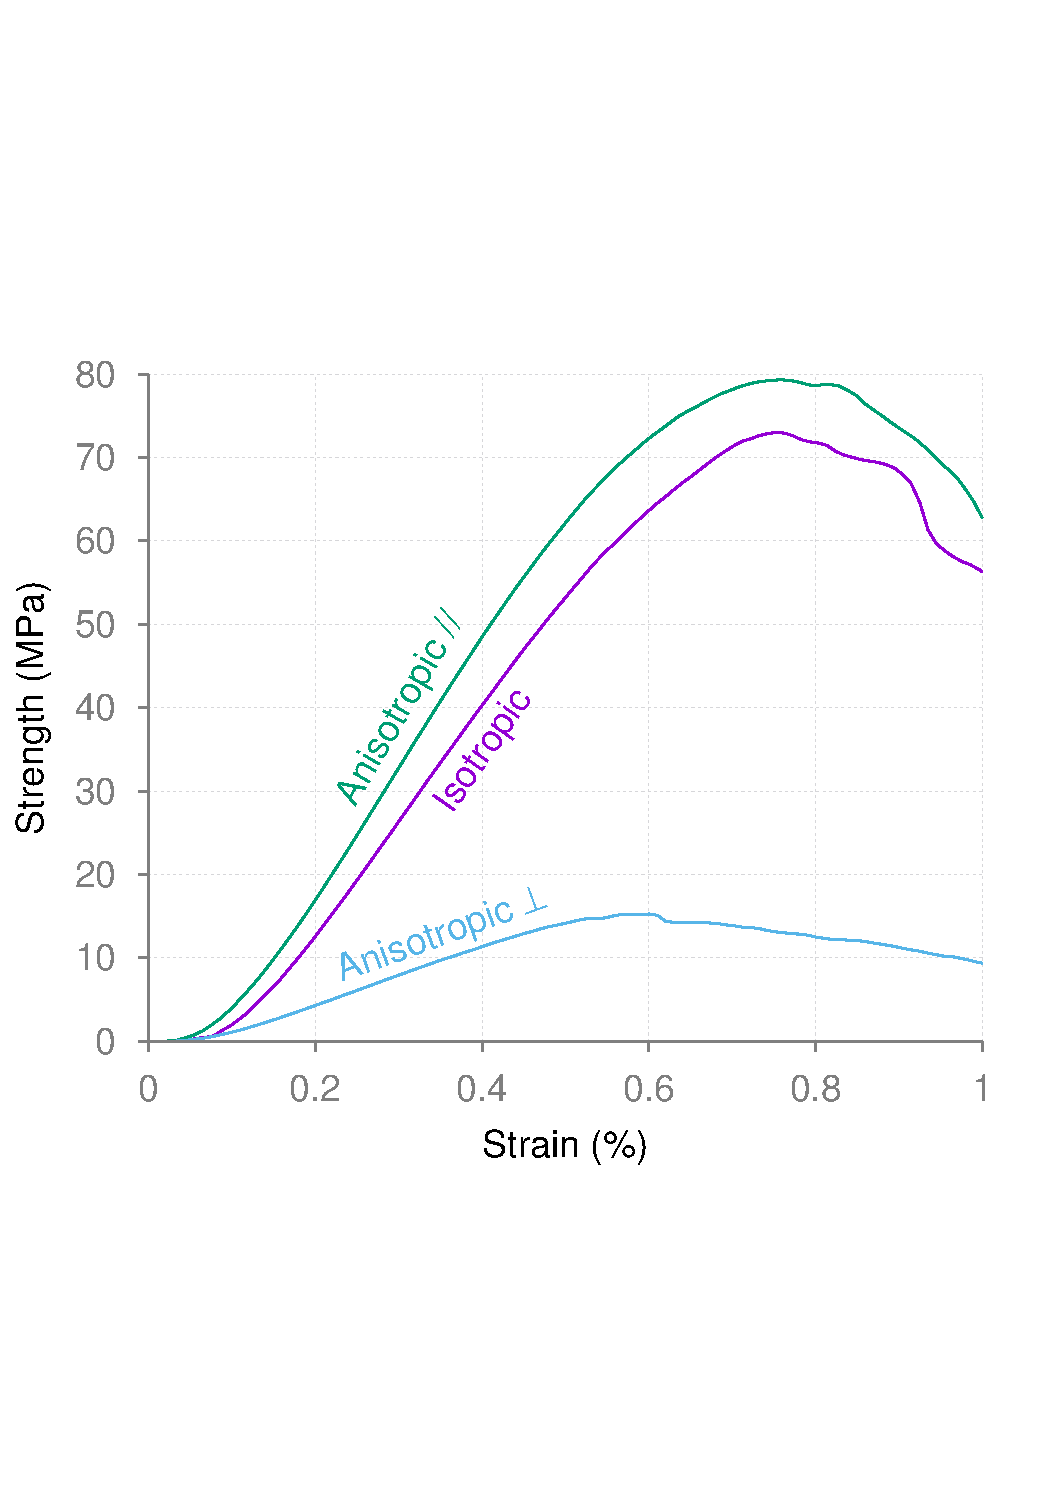
\includegraphics[width=\linewidth]{figures/sup_fig1}
		\caption{Typical response of a strain-strength curve for a numerical test on tomographic images. Total porosity of the samples are $\epsilon_\text{aniso} = 0.69$ and $\epsilon_\text{iso} = 0.62$}
	\end{figure}
	\begin{figure}[ht]
		\centering
		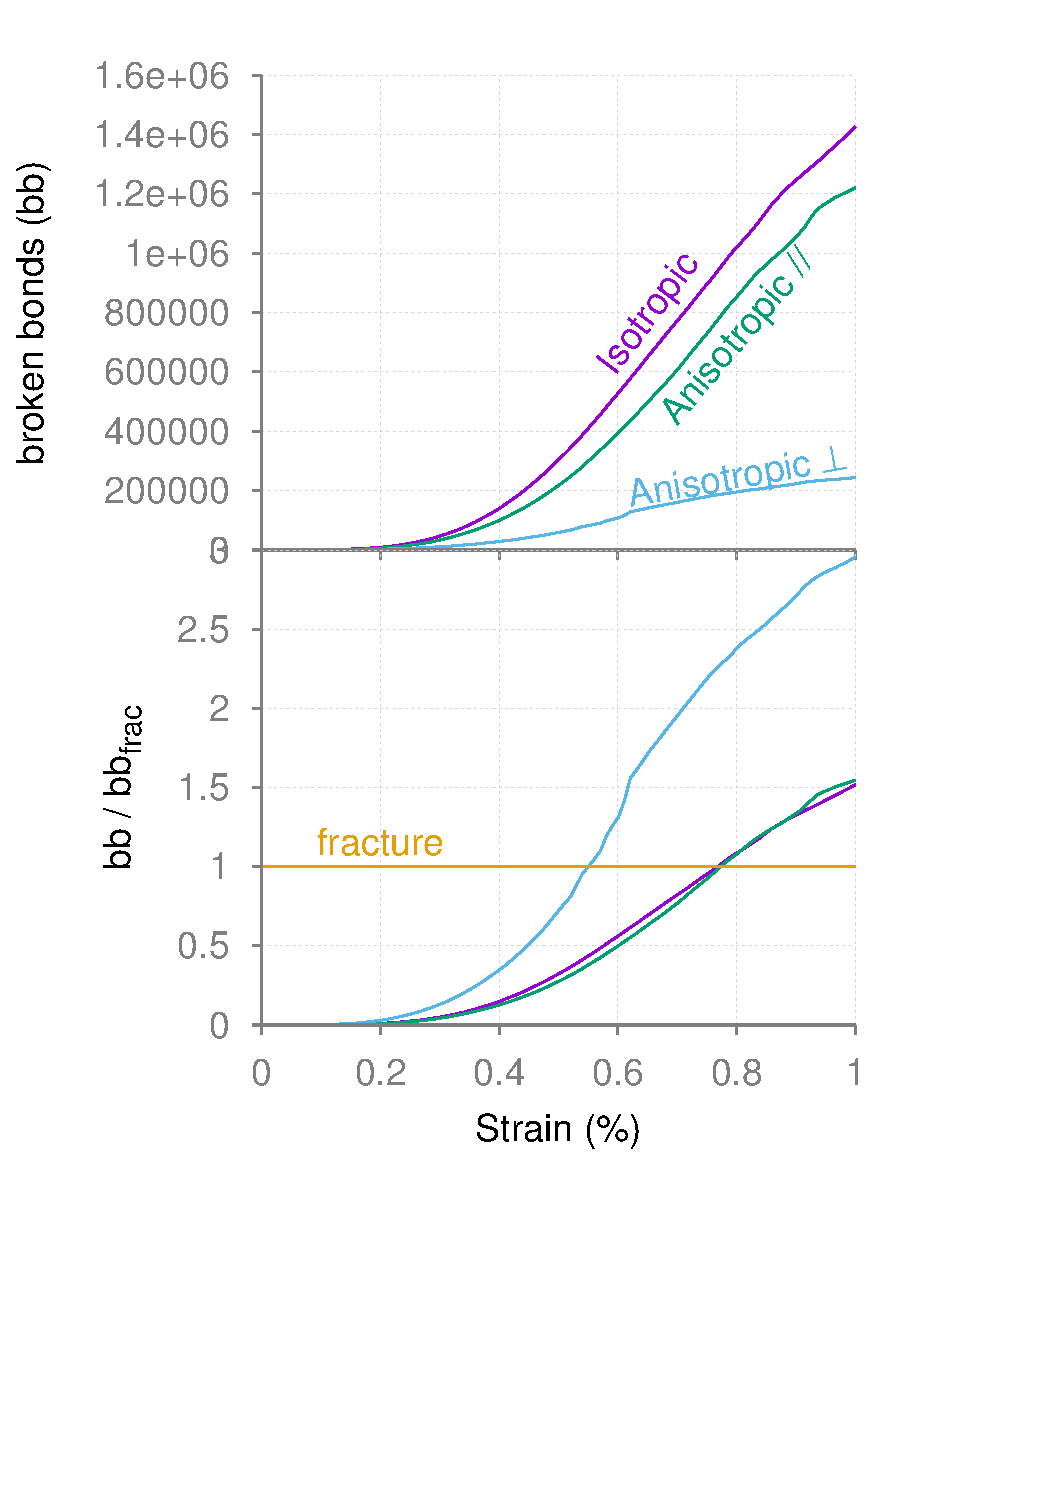
\includegraphics[width=\linewidth]{figures/sup_fig2}
		\caption{Number of broken bonds during the numerical test. Total porosity of the samples are $\epsilon_\text{aniso} = 0.69$ and $\epsilon_\text{iso} = 0.62$}
	\end{figure}
\end{document}